\documentclass[10pt,letterpaper]{beamer}

\usepackage{graphicx}
%\usepackage[spanish]{babel}
\usepackage[latin1]{inputenc}
\usepackage{listings}
\usepackage{amsmath}
\usepackage{amsfonts}
\usepackage{amsxtra}
\usepackage{amstext}
\usepackage{amssymb}
\usepackage{latexsym}
\usepackage{subfigure}
\usepackage{eurosym}
\linespread{1.2}
\usepackage{multimedia}
\usepackage{dsfont} % for \mathds{N}
\usepackage{graphicx}
\usepackage{color,colortbl}
\usepackage{multirow}
\definecolor{clearBlue}{cmyk}{0.15,0.1,0,0.1}
\usepackage{bbm}

\newcommand{\bluecell}{\cellcolor{clearBlue}}
\newtheorem{assumption}{Assumption}
\newtheorem{assumption_1}{Assumption 1: Firms Maximize Profits}
\newtheorem{assumption_2}{Assumption 2: Firms are Right on Average}
\newtheorem{assumption_3}{Assumption 3: Orthogonality}
\newcommand{\argmax}{\operatornamewithlimits{argmax}}
\newcommand{\argmin}{\operatornamewithlimits{argmin}}

%NOTE: We can uncomment the following environment in order to obtain a different style for the headings of each slide:
%\mode<presentation> {
%  \usetheme{Madrid}
%  \setbeamertemplate{navigation symbols}{}
%}

%\beamerdefaultoverlayspecification{<+->}

\hypersetup{colorlinks=true,linkcolor=red}

%NOTE: We can uncomment the following environment in order to obtain a different style for the bottom line of each slide:
%\defbeamertemplate*{footline}{my theme}
%{
%  \leavevmode%
%  \hbox{%
%  \begin{beamercolorbox}[wd=.333333\paperwidth,ht=2.25ex,dp=1ex,center]{author in head/foot}%
%    \usebeamerfont{author in head/foot}\insertshortauthor~~(\insertshortinstitute)
%  \end{beamercolorbox}%
%  \begin{beamercolorbox}[wd=.333333\paperwidth,ht=2.25ex,dp=1ex,center]{title in head/foot}%
%    \usebeamerfont{title in head/foot}\insertshorttitle
%  \end{beamercolorbox}%
%  \begin{beamercolorbox}[wd=.333333\paperwidth,ht=2.25ex,dp=1ex,right]{date in head/foot}%
%    \usebeamerfont{date in head/foot}\insertshortdate{}\hspace*{2em}
%    \insertframenumber{}\hspace*{2ex} 
%  \end{beamercolorbox}}%
%  \vskip0pt%
%}


\title[]{Identification of Discrete Choice Models Using Moment Inequalities:\\Theory and Application}
%\subtitle[]{IdentifiEstimation of Discrete Choice Problems}

\author[Morales] {Eduardo Morales}
\institute[Columbia University & Princeton University]{Columbia University \& Princeton University}
\date[]{April 2, 2012}

\AtBeginSection[] {
  \begin{frame}<beamer>
    \frametitle{Overview}
    \tableofcontents[currentsection]
  \end{frame}
}

\begin{document}

%%%%%%%%%%%%%%%%%%%%%%%%%%%%
\begin{frame}[plain]
  \titlepage
\end{frame}
%%%%%%%%%%%%%%%%%%%%%%%%%%%%
\begin{frame}
\frametitle{Topics}

\begin{itemize}
	\item Mapping between statistical and behavioral discrete choice models.
	\begin{itemize}
		\item Pakes (2010); Pakes et al. (2011); Dickstein and Morales (2012).
%		\item Ishii (2008); Ho (2009); Pakes (2010); Holmes (2011); Pakes et. al (2011); Morales (2011).
	\end{itemize}
	\item Definition and computation of alternative moment inequalities estimators.
	\begin{itemize}
		\item Chernozhukov, Hong and Tamer (2007); Andrews and Soares (2010); Pakes et al. (2011).
	\end{itemize}
\end{itemize}
\end{frame}
%%%%%%%%%%%%%%%%%%%%%%%%%%%%
\begin{frame}
\centerline{MAPPING BETWEEN STATISTICAL AND BEHAVIORAL MODELS}
\end{frame}
%%%%%%%%%%%%%%%%%%%%%%%%%%%%
\begin{frame}
\frametitle{Discrete Choice Problem}

\begin{itemize}
	\item Utility of agent $i$ for alternative $j$ is:
	\begin{equation*}
	U_{ij}=\beta x^{*}_{ij} + \nu_{ij},\qquad  j = 1,\dots,J,\quad x^{*}_{ij}\in\mathcal{X}\in R^{2}.
	\end{equation*}
	\item Choice of individual $i$ is captured in $d_{i}$ and
	\begin{equation*}
	d_{ij} = \mathbbm{1}[U_{ij}\geq U_{ij'},\text{ for $j'=1\dots,J$}].
	\end{equation*}
	\item We observe a random sample of vectors
	\begin{equation*}
	(d_{i},x_{i},z_{i})\sim\mathcal{P},\qquad i = 1,\dots,N,
	\end{equation*}
	with $x_{i1}=x^{*}_{i1}+\epsilon^{x}_{i1},$ $z_{i1}=x^{*}_{i1} + \epsilon^{z}_{i1},$ $x_{i2}=x^{*}_{i2}$.
	\item Assumptions on $(\nu_{i},\epsilon^{x}_{i1},\epsilon^{z}_{i1})$:
	\begin{itemize}
	\item structural error: $\nu_{i}\sim F_{\nu}(\nu_{i}|x_{i}^{*},\epsilon_{i1}^{x},\epsilon_{i1}^{z})$ = $F_{\nu}(\nu_{i}|x_{i}^{*})$
	\item measurement error: $\epsilon^{x}_{i1}\sim F_{\epsilon^{x}}(\epsilon_{i1}^{x}|x_{i}^{*},\epsilon_{i1}^{z},\nu_{i})$ = $F_{\epsilon^{x}}(\epsilon_{i1}^{x}|x_{i}^{*})$.
	\end{itemize}
	\item Note: we omit subindex $i$ from here onwards.
\end{itemize}
\end{frame}
%%%%%%%%%%%%%%%%%%%%%%%%%%%%
\begin{frame}
\frametitle{Example I: Estimation of Structural Parameters}
\framesubtitle{Consumer Choice Problem}

\begin{itemize}
	\item Each individual maximizes a utility function:
	\begin{equation*}
	U_{j}=\beta_{1}\mathbbm{E}[x_{j}|\mathcal{J}] +\beta_{2}p_{j}+ \nu_{j},\qquad  j = 1,\dots,J.
	\end{equation*}
	\item Instead of agent's $i$ subjective expectations, the econometrician observes both the realized values,
	\begin{equation*}
	x_{j} = \mathbbm{E}[x_{j}|\mathcal{J}] + \epsilon^{x}_{j},\text{ $\mathbbm{E}[\epsilon^{x}_{j}|\mathcal{J}]=0$,}
	\end{equation*}
	and an additional shifter of agent's $i$ expectations:
	\begin{equation*}
	z_{j} = \mathbbm{E}[x_{j}|\mathcal{J}] + \epsilon^{z}_{j}.
	\end{equation*}
	\item The expectational error corresponds to the classical measurement error in an explanatory variable (errors-in-variables).
\end{itemize}
\end{frame}
%%%%%%%%%%%%%%%%%%%%%%%%%%%%
\begin{frame}
\frametitle{Example II: Estimation of Structural Parameters}
\framesubtitle{Two-period Entry Problem}

\begin{itemize}
	\item Each firm decides where to locate a plant:
	\begin{equation*}
	U_{j}=\mathbbm{E}[R_{j}|\mathcal{J}] +\beta_{2}F_{j}+ \nu_{j},\qquad  j = 1,\dots,J.
	\end{equation*}
	\item Instead of agent's $i$ subjective expectations, the econometrician observes realized values:
	\begin{equation*}
	R_{j} = \mathbbm{E}[R_{j}|\mathcal{J}] + \epsilon^{R}_{j}.
	\end{equation*}
	The econometrician also observes $Z$ such that
	\begin{equation*}
	Z_{j} = \mathbbm{E}[R_{j}|\mathcal{J}] + \epsilon^{Z}_{j},
	\end{equation*}
	\item Similar to previous example but with structural restriction: $\beta_{1}$ = $1$.
	\item Standard application of the moment inequalities estimator:
	\begin{itemize}
		\item Ishii (2008), Ho (2009), Holmes (2011), Morales et al. (2011).
	\end{itemize}
\end{itemize}
\end{frame}
%%%%%%%%%%%%%%%%%%%%%%%%%%%%
\begin{frame}
\frametitle{Example III: Estimation of Reduced Form Parameters}
\framesubtitle{General Entry Problem}

\begin{itemize}
	\item Each firm decides where to locate a plant. Period $t$ profits of locating plant in location $j$ are:
	\begin{equation*}
	\pi_{jt} = R_{jt}-\sum_{j'=1}^{J}F_{jj'}d_{ij't-1}
	\end{equation*}
	\item The expected present value of locating plant in location $j$ is:
	\begin{align*}
	U_{jt}&=\mathbbm{E}[\pi_{jt}+\sum_{s=t+1}^{\infty}\delta^{s-t}d_{js}\pi_{js}|\mathcal{J}_{t},d_{jt}=1],\\
	&=V_{jt}-\sum_{j'=1}^{J}F_{jj'}d_{j't-1},
	\end{align*}
	with
	\begin{equation*}
	V_{jt}=\pi_{jt}+\mathbbm{E}[\sum_{s=t+1}^{\infty}\delta^{s-t}d_{js}\pi_{js}|\mathcal{J}_{t},d_{jt}=1].
	\end{equation*}
\end{itemize}
\end{frame}
%%%%%%%%%%%%%%%%%%%%%%%%%%%%
\begin{frame}
\frametitle{Example III: Estimation of Reduced Form Parameters}
\framesubtitle{General Entry Problem (cont.)}

\begin{itemize}
	\item Assume a projection of $V_{jt}$ on a set of observable covariates:
	\begin{equation*}
	V_{jt}=\beta x_{jt} + \nu_{jt},\qquad(x_{t},\nu_{t})\in\mathcal{J}_{it}.
	\end{equation*}
	\item Assume a structural form for $F_{jj'}$:
	\begin{equation*}
	F_{jj'}=\theta\|L_{j}-L_{j'}\|,
	\end{equation*}
	with $\|\cdot\|$ some measure of distance, and $L_{j}$ an indicator of location $j$.
	\item Therefore:
	\begin{equation*}
	U_{jt}=\beta x_{jt}+\theta\sum_{j'=1}^{J}\|L_{j}-L_{j'}\|d_{j't-1}+\nu_{jt}.
	\end{equation*}
	\item Additionally, we can allow for measurement error in $x_{jt}$.
\end{itemize}
\end{frame}
%%%%%%%%%%%%%%%%%%%%%%%%%%%%
\begin{frame}
\frametitle{Maximum Likelihood Estimation}

\begin{itemize}
	\item Model 1:
	\begin{itemize}
		\item Assume (up to a finite parameter vector) the distributions: 
		\begin{equation*}
		\{F_{\nu}(\nu|x^{*}), F_{\epsilon}(\epsilon|x^{*}), \mathcal{P}_{x^{*}}(x^{*})\}
		\end{equation*}
		\item The individual $i$ likelihood function is:
		\begin{equation*}
		\begin{split}
		\mathcal{L}(d|x,z)&=\mathbb{P}(d_{j}=1|x,z)\\
		&=\mathbbm{E}(\mathbbm{1}\{d_{j}=1\}|x,z)\\
		&=\mathbbm{E}(\mathbbm{E}(\mathbbm{1}\{d_{j}=1\}|x,z,x^{*})|x,z)\\
		&=\mathbbm{E}(\mathbbm{E}(\mathbbm{1}\{d_{j}=1\}|x^{*})|x,z)\\
		&=\int_{x}\Big[\int_{\nu}\mathbbm{1}\{U_{j}\geq\max_{j'\in J}\{U_{j'}\}\}dF_{\nu}(\nu|x^{*})\Big]dF_{x^{*}}(x^{*}|x,z),\\
		\end{split}
		\end{equation*}
		with
		\begin{equation*}
		U_{j}=\beta x^{*}_{j}+\nu_{j}.
		\end{equation*}
	\end{itemize}
\end{itemize}
\end{frame}
%%%%%%%%%%%%%%%%%%%%%%%%%%%%
\begin{frame}
\frametitle{Maximum Likelihood Estimation}

\begin{itemize}
	\item Model 2:
	\begin{itemize}
		\item Assume (up to a finite parameter vector) the distributions: 
		\begin{equation*}
		\{F_{\nu}(\nu|x^{*}), F_{\epsilon}(\epsilon^{x}|x^{*}), \mathcal{P}_{x^{*}}(x^{*})\}
		\end{equation*}
		such that:
		\begin{equation*}
		F_{\nu}(\nu|x^{*})=F_{\nu}(\nu),\quad\text{and}\quad F_{\epsilon}(\epsilon|x)=F_{\epsilon}(\epsilon)
		\end{equation*}
		\item The individual $i$ likelihood function is:
		\begin{equation*}
		\begin{split}
		\mathcal{L}(d|x)&=\mathbb{P}(d_{j}=1|x)\\
		&=\mathbbm{E}(\mathbbm{1}\{d_{j}=1\}|x)\\
		&=\int_{\nu+\epsilon}\mathbbm{1}\{U_{j}\geq\max_{j'\in J}\{U_{j'}\}\}dF_{\nu+\epsilon}(\nu+\epsilon^{x}),\\
		\end{split}
		\end{equation*}
		with
		\begin{equation*}
		U_{j}=\beta x_{j}+\nu_{j}-\beta\epsilon^{x}_{j}.
		\end{equation*}
	\end{itemize}
\end{itemize}
\end{frame}		
%%%%%%%%%%%%%%%%%%%%%%%%%%%%
\begin{frame}
\frametitle{Maximum Likelihood Estimation}

\begin{itemize}
	\item Model 3:
	\begin{itemize}
		\item Assume (up to a finite parameter vector) the distribution
		\begin{equation*}
		F_{\nu}(\nu|x^{*}),
		\end{equation*}
		and assume
		\begin{equation*}
		x = x^{*}.
		\end{equation*}
		\item The individual $i$ likelihood function is:
		\begin{equation*}
		\begin{split}
		\mathcal{L}(d|x)&=\mathbb{P}(d_{j}=1|x)\\
		&=\mathbbm{E}(\mathbbm{1}\{d_{j}=1\}|x)\\
		&=\mathbbm{E}(\mathbbm{1}\{d_{j}=1\}|x^{*})\\
		&=\int_{\nu}\mathbbm{1}\{U_{j}\geq\max_{j'\in J}\{U_{j'}\}\}dF_{\nu}(\nu|x^{*}),\\
		\end{split}
		\end{equation*}
		with
		\begin{equation*}
		U_{j}=\beta x^{*}_{j}+\nu_{j}.
		\end{equation*}
	\end{itemize}
\end{itemize}
\end{frame}
%%%%%%%%%%%%%%%%%%%%%%%%%%%%
\begin{frame}
\frametitle{Summary of MLE}

\begin{itemize}
	\item In words, dealing with both structural and measurement error  in MLE requires:
	\begin{itemize}
		\item Assuming both the marginal distribution of the unobserved true covariates, and the distribution of both measurement and structural error conditional on these covariates (Model 1); or,
		\item Assuming the structural error is independent of the true covariates, and the measurement error is independent of the \textit{observed} covariates (Model 2):
		\begin{itemize}
			\item Only in this case the difference between structural and measurement error is irrelevant!. We can think of a single error, $\eta$, such that:
			\begin{equation*}
			\eta = \nu + \epsilon
			\end{equation*}
			and assume a single distribution $F_{\eta}(\eta)$; or,
		\end{itemize}
		\item Assuming the distribution of the structural error conditional on the true covariates, and assuming that these are measured without error (Model 3).
	\end{itemize}
\end{itemize}
\end{frame}
%%%%%%%%%%%%%%%%%%%%%%%%%%%%
\begin{frame}
\frametitle{Moment Inequalities}
\framesubtitle{Introduction}

\begin{itemize}
	\item Given our discrete choice problem, we can derive conditional moment inequalities. A conditional moment inequality is:
	\begin{equation*}
	\mathbbm{E}[m(x,z,j,j';\beta_{0})|x,z]\geq 0,\text{ where $d_{j}$ $=$ $1$, and $j'\neq j$}.
	\end{equation*}
	\item For simplicity, in these slides we base identification on a set of unconditional moment inequalities derived for each possible value of $(x,z,j,j')$:
	\begin{equation*}
	\mathbbm{E}[m_{s}(x,z,j,j';\beta_{0})]\geq 0,\quad s=1,\dots,S.
	\end{equation*}
	\item Moment inequalities will generically lead to set identification. The identified set is:
	\begin{equation*}
	\{\beta\in\mathcal{B}:\int\sum_{s\in S}\sum_{j\in J}\sum_{j'\neq j}(\min\{m_{s}(x,z,j,j';\beta),0\}^{2})d\mathcal{P}(x,z)=0\}
	\end{equation*}
	\item We denote the identified set as $\mathcal{B}_{\mathcal{M}}(\mathcal{P})$.
\end{itemize}
\end{frame}
%%%%%%%%%%%%%%%%%%%%%%%%%%%%
\begin{frame}
\frametitle{Moment Inequalities}
\framesubtitle{Deriving Moment Inequalities from our Discrete Choice Problem: Model 1}

\begin{itemize}
	\item Assumptions: 
	\begin{equation*}
	(\epsilon^{x}_{j}, \nu_{j}) = (0,0),\quad\text{for every $j$ $\in$ $J$.}
	\end{equation*}
	\item Moment inequalities. 
	\begin{equation*}
	\mathbbm{E}[m_{s}(x,z,j,j';\beta_{0})|x,z]=\mathbbm{E}[\mathbbm{1}\{d_{j}=1\}\chi_{s}(\Delta x_{jj'}) \beta_{0}\Delta x_{jj'}|x]\geq 0,
	\end{equation*}
	where $\chi_{s}(\Delta x_{jj'})$ has the form:
	\begin{subequations}\label{eq: inst}
	\begin{align}
	\chi_{1}(\Delta x_{jj'}) &= \mathbbm{1}\{\Delta x_{1jj'}\geq 0\}\mathbbm{1}\{\Delta x_{2jj'}\geq 0\}\\
	\chi_{2}(\Delta x_{jj'}) &= \mathbbm{1}\{\Delta x_{1jj'}\geq 0\}\mathbbm{1}\{\Delta x_{2jj'}<0\}\\
	\chi_{3}(\Delta x_{jj'}) &= \mathbbm{1}\{\Delta x_{1jj'}<0\}\mathbbm{1}\{\Delta x_{2jj'}\geq 0\}\\
	\chi_{4}(\Delta x_{jj'}) &= \mathbbm{1}\{\Delta x_{1jj'}<0\}\mathbbm{1}\{\Delta x_{2jj'}<0\}.
	\end{align}
	\end{subequations}
	\item Normalization by scale: (1) $\beta_{01}=1$; (2) $\|\beta_{0}\|=1$.
	\item Completely deterministic model; very likely rejected by the data.
\end{itemize}
\end{frame}
%%%%%%%%%%%%%%%%%%%%%%%%%%%%
\begin{frame}
\frametitle{Moment Inequalities}
\framesubtitle{Deriving Moment Inequalities from our Discrete Choice Problem: Model 2}

\begin{itemize}
	\item Assumptions:
	\begin{itemize}
		\item No structural error: $\nu_{j} = 0$, for every $j$ $\in$ $J$;
		\item Measurement error indep. of true covariate: $F_{\epsilon}[\epsilon^{x}_{1}|x^{*}]$ = $F_{\epsilon}[\epsilon^{x}_{1}]$
		\begin{itemize}
			\item No parametric assumption on $F_{\epsilon}[\epsilon^{x}_{1}]$ needed.
		\end{itemize}
		\item Additional indicator of the covariate measured with error: $z_{1}$.
	\end{itemize}
	\item Moment inequalities.
	\begin{align*}
	\mathbbm{E}[\mathbbm{1}\{d_{j}=1\}\chi_{s}(\Delta z_{1jj'},\Delta x_{2jj'})\beta_{0}\Delta x^{*}_{jj'}|x,z]&\geq 0,\\
	\mathbbm{E}[\mathbbm{1}\{d_{j}=1\}\chi_{s}(\Delta z_{1jj'},\Delta x_{2jj'})(\beta_{0}\Delta x_{jj'}-\beta_{0}\Delta \epsilon^{x}_{1jj'})|x,z]&\geq 0,\\
	\mathbbm{E}[\mathbbm{1}\{d_{j}=1\}\chi_{s}(\Delta z_{1jj'},\Delta x_{2jj'})\beta_{0}\Delta x_{jj'}|x,z]&\geq 0,
	\end{align*}
	with
	\begin{align*}
	\chi_{1}(\Delta z_{1jj'},\Delta x_{2jj'}) &= \mathbbm{1}\{\Delta z_{1jj'}\geq 0\}\mathbbm{1}\{\Delta x_{2jj'}\geq 0\},\\
	\chi_{2}(\Delta z_{1jj'},\Delta x_{2jj'}) &= \mathbbm{1}\{\Delta z_{1jj'}\geq 0\}\mathbbm{1}\{\Delta x_{2jj'}<0\},\\
	\chi_{3}(\Delta z_{1jj'},\Delta x_{2jj'}) &= \mathbbm{1}\{\Delta z_{1jj'}<0\}\mathbbm{1}\{\Delta x_{2jj'}\geq 0\},\\
	\chi_{4}(\Delta z_{1jj'},\Delta x_{2jj'}) &= \mathbbm{1}\{\Delta z_{1jj'}<0\}\mathbbm{1}\{\Delta x_{2jj'}<0\}.
	\end{align*}
%	\item Normalization by scale: (1) $\beta_{01}=1$; (2) $\|\beta_{0}\|=1$.
\end{itemize}
\end{frame}
%%%%%%%%%%%%%%%%%%%%%%%%%%%%
\begin{frame}
\frametitle{Moment Inequalities}
\framesubtitle{Deriving Moment Inequalities from our Discrete Choice Problem: Model 3}

\begin{itemize}
	\item Assumptions:
	\begin{itemize}
		\item No structural error: $\nu_{j} = 0$, for every $j$ $\in$ $J$;
		\item Measurement error indep. of true covariate: $F_{\epsilon}[\epsilon^{x}_{1}|x^{*}]$ = $F_{\epsilon}[\epsilon^{x}_{1}]$;
		\begin{itemize}
			\item No parametric assumption on $F_{\epsilon}[\epsilon^{x}_{1}]$ needed.
		\end{itemize}
		\item Structural restriction: $\beta_{01}$ = $1$.
	\end{itemize}
	\item Moment inequalities. 
	\begin{align*}
	\mathbbm{E}[\mathbbm{1}\{d_{j}=1\}\chi_{s}(\Delta x_{2jj'})\beta_{0}\Delta x^{*}_{jj'}|x]&\geq 0,\\
	\mathbbm{E}[\mathbbm{1}\{d_{j}=1\}\chi_{s}(\Delta x_{2jj'})(\beta_{0}\Delta x_{jj'}-\beta_{0}\Delta \epsilon^{x}_{1jj'})|x]&\geq 0,\\
	\mathbbm{E}[\mathbbm{1}\{d_{j}=1\}\chi_{s}(\Delta x_{2jj'})\beta_{0}\Delta x_{jj'}]&\geq 0,
	\end{align*}
	with
	\begin{align*}
	\chi_{1}(\Delta x_{2jj'}) &= \mathbbm{1}\{\Delta x_{2jj'}\geq 0\},\\
	\chi_{2}(\Delta x_{2jj'}) &= \mathbbm{1}\{\Delta x_{2jj'}<0\}
	\end{align*}
	\item No need to normalize by scale.
\end{itemize}
\end{frame}
%%%%%%%%%%%%%%%%%%%%%%%%%%%%
\begin{frame}
\frametitle{Moment Inequalities}
\framesubtitle{Deriving Moment Inequalities from our Discrete Choice Problem: Model 4}

\begin{itemize}
	\item Assumptions:
	\begin{itemize}
		\item Structural error organized in nests:
		\begin{equation*}
		\nu_{j} - \nu_{j'} = \left\{
		\begin{array}{ll}
		0 & \text{if $G(j)=G(j')$},\\
		\mathbbm{R} & \text{if $G(j)\neq G(j')$},\\
		\end{array} \right.
		\end{equation*}
		where $G(j)$ denotes a particular subset of $J$.\\
		\begin{itemize}
			\item No parametric assumption on $F_{\nu}[\nu|x]$ needed.
		\end{itemize}
		\item No measurement error.
	\end{itemize}
	\item Moment inequalities.
	\begin{align*}
	\mathbbm{E}[\mathbbm{1}\{d_{j}=1\}\mathbbm{1}\{G(j)=G(j')\}\chi_{s}(\Delta x_{jj'})(\beta_{0}\Delta x_{jj'}+\Delta\nu_{jj'})|x]\geq 0,\\
	\mathbbm{E}[\mathbbm{1}\{d_{j}=1\}\mathbbm{1}\{G(j)=G(j')\}\chi_{s}(\Delta x_{jj'}) \beta_{0}\Delta x_{jj'}|x]\geq 0,
	\end{align*}
	%\item Normalization by scale: (1) $\beta_{01}=1$; (2) $\|\beta_{0}\|=1$.
	\item Trivial to allow for measurement error indep. of the true covariate. 
	\begin{itemize}
		\item use an additional indicator $z_{1}$ (as in Model 2); or,
		\item impose $\beta_{01}$ $=$ $1$ as a structural assumption (as in Model 3).
	\end{itemize}
\end{itemize}
\end{frame}
%%%%%%%%%%%%%%%%%%%%%%%%%%%%
\begin{frame}
\frametitle{Moment Inequalities}
\framesubtitle{Deriving Moment Inequalities from our Discrete Choice Problem: Model 5}

\begin{itemize}
	\item Assumptions:
	\begin{itemize}
		\item Ordered choice model:
		\begin{equation*}
		\nu_{j} = j\eta,\quad\text{and}\quad F_{\eta}[\eta|x]=F_{\eta}[\eta],
		\end{equation*}
		with $\mathbbm{E}[\eta]=0$.
		\begin{itemize}
			\item No parametric assumption on $F_{\eta}[\eta|x]$ needed.
		\end{itemize}
		\item No measurement error.
	\end{itemize}
	\item Moment inequalities.
	\begin{align*}
	\mathbbm{E}[\mathbbm{1}\{d_{j}=1\}\mathbbm{1}\{j-j'=1\}\chi_{s}(\Delta x_{jj'})(\beta_{0}\Delta x_{jj'}+\Delta\nu_{jj'})|x]\geq 0,\\
	\mathbbm{E}[\mathbbm{1}\{d_{j}=1\}\mathbbm{1}\{j-j'=1\}\chi_{s}(\Delta x_{jj'})(\beta_{0}\Delta x_{jj'}+\eta)|x]\geq 0,\\
	\mathbbm{E}[\mathbbm{1}\{d_{j}=1\}\mathbbm{1}\{j-j'=1\}\chi_{s}(\Delta x_{jj'})\beta_{0}\Delta x_{jj'}|x]\geq 0.
	\end{align*}
	%\item Normalization by scale: (1) $\beta_{01}=1$; (2) $\|\beta_{0}\|=1$.
	\item Trivial to allow for measurement error indep. of the true covariate. 
	\begin{itemize}
		\item use an ``instrument'' $z_{1}$, and assume $F_{\eta}[\eta|x^{*},\epsilon^{z}_{1}]=F_{\eta}[\eta]$;
		\item impose $\beta_{01}$ $=$ $1$, and assume $F_{\eta}[\eta|x^{*}]=F_{\eta}[\eta]$.
	\end{itemize}
\end{itemize}
\end{frame}
%%%%%%%%%%%%%%%%%%%%%%%%%%%%
\begin{frame}
\frametitle{Moment Inequalities}
\framesubtitle{Deriving Moment Inequalities from our Discrete Choice Problem: Additional Models}

See Dickstein and Morales (2012) (\textit{to be posted soon}) for guidance on how to build moment inequalities for the following models:
	\begin{itemize}
		\item Model 6:
		\begin{itemize}
			\item Assume a parametric distribution for $\nu_{i}$: $F_{\nu}[\nu|x;\sigma]$
			\item Allow for distribution free measurement error in two cases:
			\begin{itemize}
				\item multiple indicator assumption; 
				\item fixed parameter on the variable measured with error.
			\end{itemize}
		\end{itemize}
		\item Model 7:
		\begin{itemize}
			\item Assume $\nu_{i}$ is distributed independently of $x$.
			\begin{itemize}
				\item No parametric assumption on $F_{\nu}[\nu|x]$ needed.
			\end{itemize}
			\item Allow for distribution free measurement error in two cases:
			\begin{itemize}
				\item multiple indicator assumption; 
				\item fixed parameter on the variable measured with error.
			\end{itemize}
		\end{itemize}	
	\end{itemize}
\end{frame}
%%%%%%%%%%%%%%%%%%%%%%%
\begin{frame}
\frametitle{Summary of Moment Inequalities}

\begin{itemize}
	\item In words, dealing with both structural and measurement error in Moment Inequalities requires:
	\begin{itemize}
		\item In order to deal with measurement error, we may apply any of the usual IV solutions to measurement error problems in linear regression models. In particular, no parametric assumption on its distribution function is needed.
		\item In order to deal with structural error, one needs to:
		\begin{itemize}
			\item Assume it away; or,
			\item Assume that it is an individual effect common to a subset of choices; or,
			\item Assume a parametric distribution on it; or,
			\item Assume that it is distributed independently of $x$ (no parametric assumption needed), or,
			\item In the special case of an ordered choice model, assume that it increases in an individual specific constant as the choice gets bigger.
		\end{itemize}
	\end{itemize}
\end{itemize}
\end{frame}
%%%%%%%%%%%%%%%%%%%%%%%%
\begin{frame}
\centerline{ALTERNATIVE MOMENT INEQUALITIES ESTIMATORS:}
\centerline{DEFINITION AND COMPUTATION}
\end{frame}
%%%%%%%%%%%%%%%%%%%%%%%%
\begin{frame}
\frametitle{Identified Set}

\begin{itemize}
	\item Moment inequalities will generically lead to set identification. Given a set $S$ of moment inequalities, the identified set is:
	\begin{equation*}
	\Theta^{S}=\argmin_{\theta}\sum_{s=1}^{S}\Big(\min\big\{0,\mathbbm{E}[m_{s}(Y,X,Z;\theta)]\big\}\Big)^{2}
	\end{equation*}
	\begin{figure}[h!]
	\begin{center}
	\subfigure{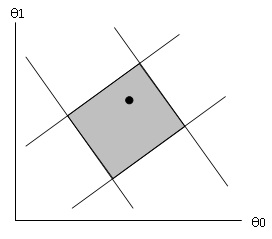
\includegraphics[scale=0.65]{Figure_1.jpg}}
	\subfigure{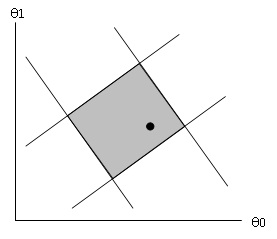
\includegraphics[scale=0.65]{Figure_2.jpg}}
	\end{center}
	\end{figure}	
\end{itemize}
\end{frame}
%%%%%%%%%%%%%%%%%%%%%%%%
\begin{frame}
\frametitle{Steps for Estimation}

\begin{itemize}
	\item Step 1: Estimate the identified set given sample moments.
	\item Step 2: Perform inference on one or more of the following parameters:
	\begin{itemize}
		\item Interval contained in the identified set: Pakes, Porter, Ho and Ishii (2011).
		\item Identified set: Chernozhukov, Hong and Tamer (Econometrica, 2007).
		\item True parameter vector: Andrews and Soares (Econometrica, 2010).
	\end{itemize}
\end{itemize}
\end{frame}
%%%%%%%%%%%%%%%%%%%%%%%%
\begin{frame}[label=estset]
\frametitle{Estimation of the Identified Set}

\begin{itemize}
	\item Estimation is based on the sample analogue of the moment inequalities:
	\begin{equation*}
	\overline{m}_{I,s}(\theta)=\frac{1}{I}\sum_{i=1}^{I}m_{s}(Y_{i},X_{i},Z_{i};\theta)
	\end{equation*}
	\begin{figure}[h!]
	\begin{center}
	\subfigure[Case 1]{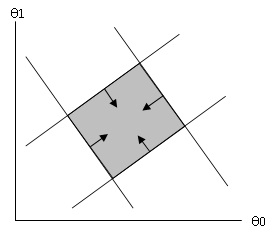
\includegraphics[scale=0.65]{Figure_3.jpg}}
	\subfigure[Case 2]{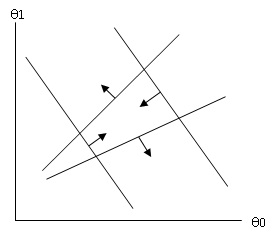
\includegraphics[scale=0.65]{Figure_4.jpg}}
	\end{center}
	\end{figure}	
\end{itemize}
\hyperlink{estsetb}{\beamerbutton{Back}}
\end{frame}
%%%%%%%%%%%%%%%%%%%%%%%%
\begin{frame}
\frametitle{Estimation of the identified set}

\begin{itemize}
	\item Two possible criterion functions to define the estimated set:
	\begin{itemize}
		\item Unweighted criterion function:
		\begin{equation*}
		\hat{\Theta}^{S}_{I} = \argmin_{\theta}\sum_{s=1}^{S}\Big(\min\{0,\overline{m}_{I,s}(\theta)\}\Big)^{2}
		\end{equation*}
		\item Weighted criterion function:
		\begin{equation*}
		\hat{\Theta}^{S}_{I} = \argmin_{\theta}\sum_{s=1}^{S}\Big(\min\{0,\Big[\frac{\overline{m}_{I,s}(\theta)}{\hat{\sigma}^{2}_{I,s}(\theta)}\Big]\}\Big)^{2},
		\end{equation*}
		with
		\begin{equation*}
		\hat{\sigma}^{2}_{I,s}(\theta)=\frac{1}{I}\sum_{i=1}^{I}(m_{s}(Y_{i},X_{i},Z_{i};\theta)-\overline{m}_{I,s}(\theta))^{2}
		\end{equation*}
	\end{itemize}
	\item They both generate the same estimated set in Case 1. They may generate different estimated sets in Case 2. The weighting lessens the influence of sample moments that have high variance (likely to be further away from their population analogues).
\end{itemize}
\end{frame}
%%%%%%%%%%%%%%%%%%%%%%%%
\begin{frame}
\frametitle{Computation of the estimated set}

\begin{itemize}
	\item We characterize the set $\hat{\Theta}^{S}_{I}$ by finding its boundaries along any linear combination of the dimensions of vector $\theta$.
	 \item If the moment functions $\{\overline{m}_{I,s}(\theta ): s=1,\dots,S\}$ are linear in $\theta$, use linear programming to find the extremum 
	\begin{equation}
	\begin{split}
	& \max_{\theta}\quad f\cdot \theta \\
	& \quad \text{s.t.} \\
	& \quad \overline{m}_{I,s}(\theta )\geq 0,\text{ for }s=1,...,S.
	\label{eq: optvert}
	\end{split}
	\end{equation}
	\item If we want to find the maximum and minimum of our two-dimensional parameter $\theta$, we use:
	\begin{equation*}
	f=\{[1,0],[-1,0],[0,1],[0,-1]\}.
	\end{equation*}
\end{itemize}
\end{frame}
%%%%%%%%%%%%%%%%%%%%%%%%
\begin{frame}
\frametitle{Computation of the estimated set}

\begin{itemize}
	\item If there is no value of $\theta$ that verifies all the constraints, $\hat{\Theta}^{S}_{I}$ will then be a singleton.
	\item This singleton is the outcome of the following nonlinear optimization problem:
	\begin{equation*}
	\hat{\Theta}^{S}_{I} = \argmin_{\theta}\sum_{s=1}^{S}\Big(\min\{0,\Big[\frac{\overline{m}_{I,s}(\theta)}{\hat{\sigma}^{2}_{I,s}(\theta)}\Big]\}\Big)^{2}.
	\end{equation*}
	\item It is suggested to use the \textit{KNITRO} nonlinear optimzation package from Matlab via \textit{ktrlink}.
\end{itemize}
\end{frame}
%%%%%%%%%%%%%%%%%%%%%%%%
\begin{frame}
\frametitle{Computation of the estimated set: example}

\begin{itemize}
	\item Sample moments:
	\begin{eqnarray*}
	900-\theta _{0}(-2)-\theta _{1}(60) &\geq &0 \\
	-900-\theta _{0}(2)-\theta _{1}(-55) &\geq &0 \\
	200-\theta _{0}(1)-\theta _{1}(9) &\leq &0 \\
	-200-\theta _{0}(-1)-\theta _{1}(-11) &\leq &0
	\end{eqnarray*}
\end{itemize}
\end{frame}
%%%%%%%%%%%%%%%%%%%%%%%%%
\begin{frame}
\frametitle{Computation of the estimated set: example}

\begin{figure}[h!]
\begin{center}
\subfigure{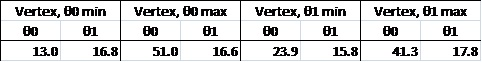
\includegraphics[scale=0.65]{Figure_5.jpg}}
\subfigure{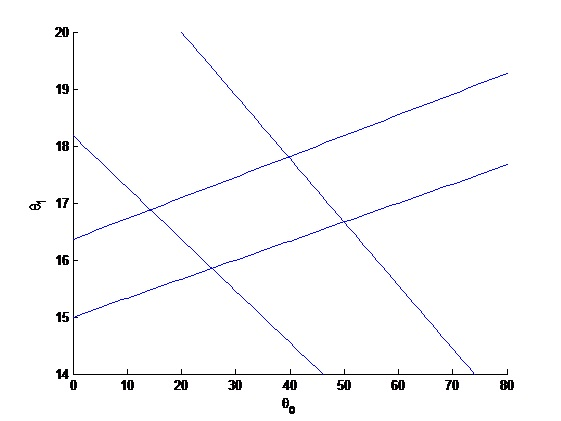
\includegraphics[scale=0.6]{Figure_6.jpg}}
\end{center}
\end{figure}	
\end{frame}
%%%%%%%%%%%%%%%%%%%%%%%%%
\begin{frame}
\frametitle{Inference: General Intuition}

\begin{itemize}
	\item Consider we want to test the null hypothesis: $H_{0}: \theta=\theta_{0}$.
	\item We use the following statistic:
	\begin{equation*}
	T_{I}(\theta_{0})=\sum_{s=1}^{S}\Big(\min\{0,\Big[\frac{\overline{m}_{I,s}(\theta_{0})}{\hat{\sigma}^{2}_{I,s}(\theta_{0})}\Big]\}\Big)^{2}.
	\end{equation*}
	\item The finite-sample null distribution of $T_{I}(\theta_{0})$ depends on the degree of \textit{slackness} of the moment inequalities (the population moments). That is, it depends on how much greater than 0 is
	\begin{equation*}
	\mathbbm{E}[m_{s}(Y_{i},X_{i},Z_{i};\theta)],\quad\text{for $s=1,\dots,S$}.
	\end{equation*}
	\item The distribution of $T_{I}(\theta_{0})$ is stochastically larger the more moments are equal to 0 at $\theta_{0}$ (the population moments).
	\item As the distribution of $T_{I}(\theta_{0})$ gets stochastically larger, the probability of rejecting $H_{0}$ decreases.
\end{itemize}
\end{frame}
%%%%%%%%%%%%%%%%%%%%%%%%%
\begin{frame}
\frametitle{Inference: General Intuition}

\begin{itemize}
	\item Therefore, it is key to infer whether a population moment binds at a particular value $\theta_{0}$. This inference is based on slackness factors computed for each moment: $SF_{I,s}(\theta_{0})$. 
	\item Three possible slackness factors proposed in the literature:
	\begin{itemize}
		\item Assume that all the $S$ moments are binding at $\theta_{0}$: $SF_{I,s}=0$. This yields the most conservative test.
		\item Moment Selection: assume a moment is asymptotically binding if the sample analogue takes a value larger than a threshold.
		\begin{equation*}
		SF^{MS}_{I,s}(\theta_{0})=\mathbbm{1}\{\sqrt{n}(\frac{\overline{m}_{I,s}(\theta_{0})}{\hat{\sigma }_{I,s}(\theta_{0})})\leq\sqrt{2\ln (\ln (n))}\}
		\end{equation*}
		\item Shifted Mean: shift each moment proportionately to how far away from binding it is in the sample.
		\begin{equation*}
		SF^{SM}_{I,s}(\theta_{0})=(\frac{\overline{m}_{I,s}(\theta_{0})}{\hat{\sigma}_{I,s}(\theta_{0})})(\frac{1}{\sqrt{2\ln(\ln (n))}})\mathbbm{1}\{\frac{\overline{m}_{I,s}(\theta_{0})}{\hat{\sigma}_{I,s}(\theta_{0})}>0\}
		\end{equation*}
	\end{itemize}
\end{itemize}
\end{frame}
%%%%%%%%%%%%%%%%%%%%%%%%%
\begin{frame}[label=estsetb]
\frametitle{Inference for an Interval}

\begin{itemize}
	\item This procedure is based on Pakes, Porter, Ho, and Ishii (2011).
	\item Objective: build confidence intervals for the vertices of the estimated set, and use the outer bounds to form a unique confidence interval.
	\item We need four elements for inference:
	\begin{itemize}
		\item Vertices of the estimated set.
		\begin{itemize}
			\item We collect these from the computation of the estimated set.
		\end{itemize}
		\item Approximation to the asymptotic distribution of all the (weighted) moments recentered at zero.
		\item Jacobian of the moments.
		\item Slackness factors.
	\end{itemize}
	\item Once we have this four elements, we perform an optimization very close to that one in equation \eqref{eq: optvert}.
\end{itemize}
\hyperlink{estset}{\beamerbutton{Est.Set}}
\end{frame}
%%%%%%%%%%%%%%%%%%%%%%%%%
\begin{frame}
\frametitle{Inference for an Interval}

\begin{itemize}
	\item Approximation to asymptotic distribution of all the recentered moments.
	\begin{itemize}
		\item As long as the CLT applies, we just need to draw $r=1,...,R$ times from a multivariate normal with zero mean, and
	covariance equal to the variance of the weighted moments
		\item How to do this?
		\begin{itemize}
			\item Take $R$ standard normal draws.
			\item Premultiply each draw by the Cholesky decomposition of the correlation matrix evaluated at the vertex of interest, $\widehat{\Omega}_{I,S}(\hat{\theta})$:
			\begin{equation*}
			\widehat{\Omega }_{I,S}(\hat{\theta})=diag(\widehat{\Sigma}_{I,S}(\hat{\theta}))^{-\frac{1}{2}}\widehat{\Sigma}_{I,S}(\hat{\theta})diag(\widehat{\Sigma}_{I,S}(\hat{\theta}))^{-\frac{1}{2}}.
			\end{equation*}
			\item Result: 
			\begin{equation*}
			q_{r}(\hat{\theta})=chol(\widehat{\Omega}_{n}(\hat{\theta}))N(0_{S},I_{S}).
			\end{equation*}
		\end{itemize}
	\end{itemize}
\end{itemize}
\end{frame}
%%%%%%%%%%%%%%%%%%%%%%%%%
\begin{frame}
\frametitle{Inference for an Interval}

\begin{itemize}
	\item Jacobian of the moments.
	\begin{itemize}
		\item Compute the Jacobian of the unweighted moments, $\overline{m}_{I,s}(\theta)$, and evaluate the result at the vertex of interest:
		\begin{equation*}
		\nabla_{\theta}\overline{m}_{I,s}(\theta)|_{\hat{\theta}}=\nabla_{\theta}\Big\{\frac{1}{I}\sum_{i=1}^{I}\sum_{j\in J}\sum_{j'\neq j}\mathbbm{1}\{Y_{i}=j\}h_{s}(Z_{i})(g(X_{j};\theta)-g(X_{j'};\theta))\Big\}\Big|_{\hat{\theta}}
		\end{equation*}
		\item Reweight the elements of the Jacobian using the diagonal elements of the covariance matrix of the unweighted moments, evaluated at the vertex of interest:
		\begin{equation*}
		\widehat{\Gamma}_{I,S}(\hat{\theta})=diag(\widehat{\Sigma}_{I,S}(\hat{\theta}))^{-\frac{1}{2}}\Big(\nabla_{\theta}\overline{m}_{I,S}(\theta)|_{\hat{\theta}}\Big)'
		\end{equation*}
	\end{itemize}
\end{itemize}
\end{frame}
%%%%%%%%%%%%%%%%%%%%%%%%%
\begin{frame}
\frametitle{Inference for an Interval}

\begin{itemize}
	\item Evaluate the slackness factor at the vertex of interest and normalize by $\sqrt{I}$.
	\begin{itemize}
		\item We could use either $SF^{MS}_{I,s}$ or $SF^{SM}_{I,s}$.\\
		The option described in Pakes, Porter, Ho, and Ishii (2011) is Shifted Mean:
		\begin{equation*}
		SF^{SM}_{I,s}(\hat{\theta})\sqrt{I} =(\frac{\overline{m}_{I,s}(\hat{\theta})}{\hat{\sigma}_{I,s}(\hat{\theta})})(\frac{1}{\sqrt{2\ln(\ln (n))}})\mathbbm{1}\{\frac{\overline{m}_{I,s}(\hat{\theta})}{\hat{\sigma}_{I,s}(\hat{\theta})}>0\}\sqrt{I}
		\end{equation*}
	\end{itemize}
\end{itemize}
\end{frame}
%%%%%%%%%%%%%%%%%%%%%%%%%
\begin{frame}
\frametitle{Inference for an Interval}

\begin{itemize}
	\item Compute the following linear programing problem for each draw $r$ and each vertex $\hat{\theta}$:
	\begin{equation}
	\begin{split}
	&\theta_{r}=\max_{\theta}\quad f\cdot\sqrt{I}(\hat{\theta}-\theta)\\
	& \quad \text{s.t.}\\
	& \quad\widehat{\Gamma}_{I,S}(\hat{\theta})\sqrt{I}(\hat{\theta}-\theta)+q_{r}(\hat{\theta})+SF^{SM}_{I,S}(\hat{\theta})\sqrt{I}\geq 0
	\label{eq: simvert}
	\end{split}
	\end{equation}
	\item As before, if we want to find the maximum and minimum of our two-dimensional parameter $\theta$, we use:
	\begin{equation*}
	f=\{[1,0],[-1,0],[0,1],[0,-1]\}.
	\end{equation*}
	In equation \eqref{eq: simvert}, we should be careful to use the estimated vertex $\hat{\theta}$ that corresponds to each vector $f$.
	\item We obtain $R$ draws of the asymptotic distribution of each of the estimated vertices of the estimated set.
\end{itemize}
\end{frame}
%%%%%%%%%%%%%%%%%%%%%%%%%
\begin{frame}
\frametitle{Inference for an Interval}

\begin{itemize}
	\item For each pair of vertices corresponding to a given dimension $d$ of $\theta$.
	\begin{itemize}
		\item For the min vertex, take the $\alpha/2$ quantile of the set of simulated vertices, $\theta_{r}$, $r=1,\dots,R$. Denote this number:
		\begin{equation*}
		\underline{\theta}_{d,\alpha/2}.
		\end{equation*}
		\item For the max vertex, take the $(1-\alpha/2)$ quantile of the set of simulated vertices, $\theta_{r}$, $r=1,\dots,R$
		\begin{equation*}
		\overline{\theta}_{d,1-\alpha/2}.
		\end{equation*}
	\end{itemize}
	\item The confidence interval for $\theta$ in the dimension $d$ with significance level $\alpha$ is:
	\begin{equation*}
	(\underline{\theta}_{d,\alpha/2},\overline{\theta}_{d,\alpha/2}).
	\end{equation*}
\end{itemize}
\end{frame}
%%%%%%%%%%%%%%%%%%%%%%%%%
\begin{frame}
\frametitle{Inference for an Interval: Example}

\begin{figure}[h!]
\begin{center}
\subfigure{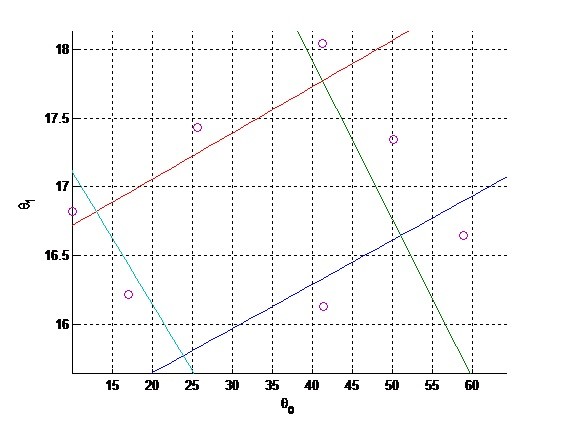
\includegraphics[scale=0.65]{Figure_7.jpg}}
\end{center}
\end{figure}	
\end{frame}
%%%%%%%%%%%%%%%%%%%%%%%%%
\begin{frame}
\frametitle{Inference for an Interval: Example}

\begin{figure}[h!]
\begin{center}
\subfigure{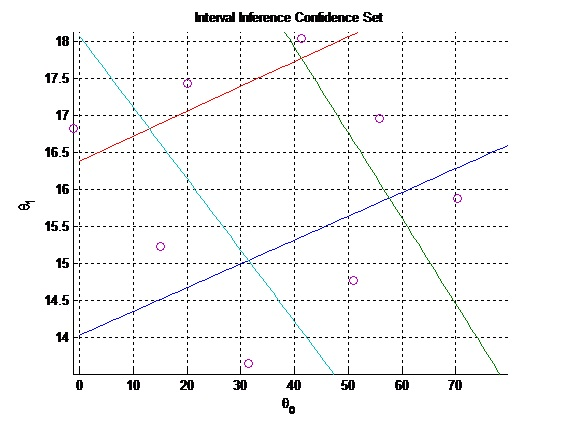
\includegraphics[scale=0.65]{Figure_8.jpg}}
\end{center}
\end{figure}	
\end{frame}
%%%%%%%%%%%%%%%%%%%%%%%%%
\begin{frame}
\frametitle{Set/Point Inference: General Intuition}

\begin{itemize}
	\item The estimation of confidence intervals for the true parameter and for the identified set are based on the inversion of an Anderson-Rubin T statistic.
	\item General steps in the algorithm:
	\begin{enumerate}
		\item Define $\theta$ grids, $\widehat{\Theta}_{I}^{Grid}$ and $\widehat{\Theta}_{I}^{\epsilon}$, where $\widehat{\Theta}_{I}^{\epsilon}\subset 
\widehat{\Theta }_{I}^{Grid}$.
		\item Calculate $T_{r}(\theta)$, at a set of points in either $\widehat{\Theta }_{I}^{Grid}$ or $\widehat{\Theta}_{I}^{\epsilon}$ depending on whether the
focus of inference is the identified set or the true value of the parameter.
		\item Determine a critical value as a quantile of $T_{r}(\theta)$ for $r=1,...,R$
		\item Calculate $T^{obs}(\theta)$ at each $\theta\in\widehat{\Theta }_{I}^{Grid}$ with the observed data for all moments.
		\item Define the confidence set as those $\theta$ points where $T^{obs}(\theta)$ falls below the critical value.
	\end{enumerate}
\end{itemize}
\end{frame}
%%%%%%%%%%%%%%%%%%%%%%%%%
\begin{frame}
\frametitle{Forming the Grids: $\widehat{\Theta}_{I}^{Grid}$ and $\widehat{\Theta}_{I}^{\epsilon}$}

$\widehat{\Theta}_{I}^{\epsilon}\subset \widehat{\Theta}_{I}^{Grid}$

\begin{figure}[h!]
\begin{center}
\subfigure{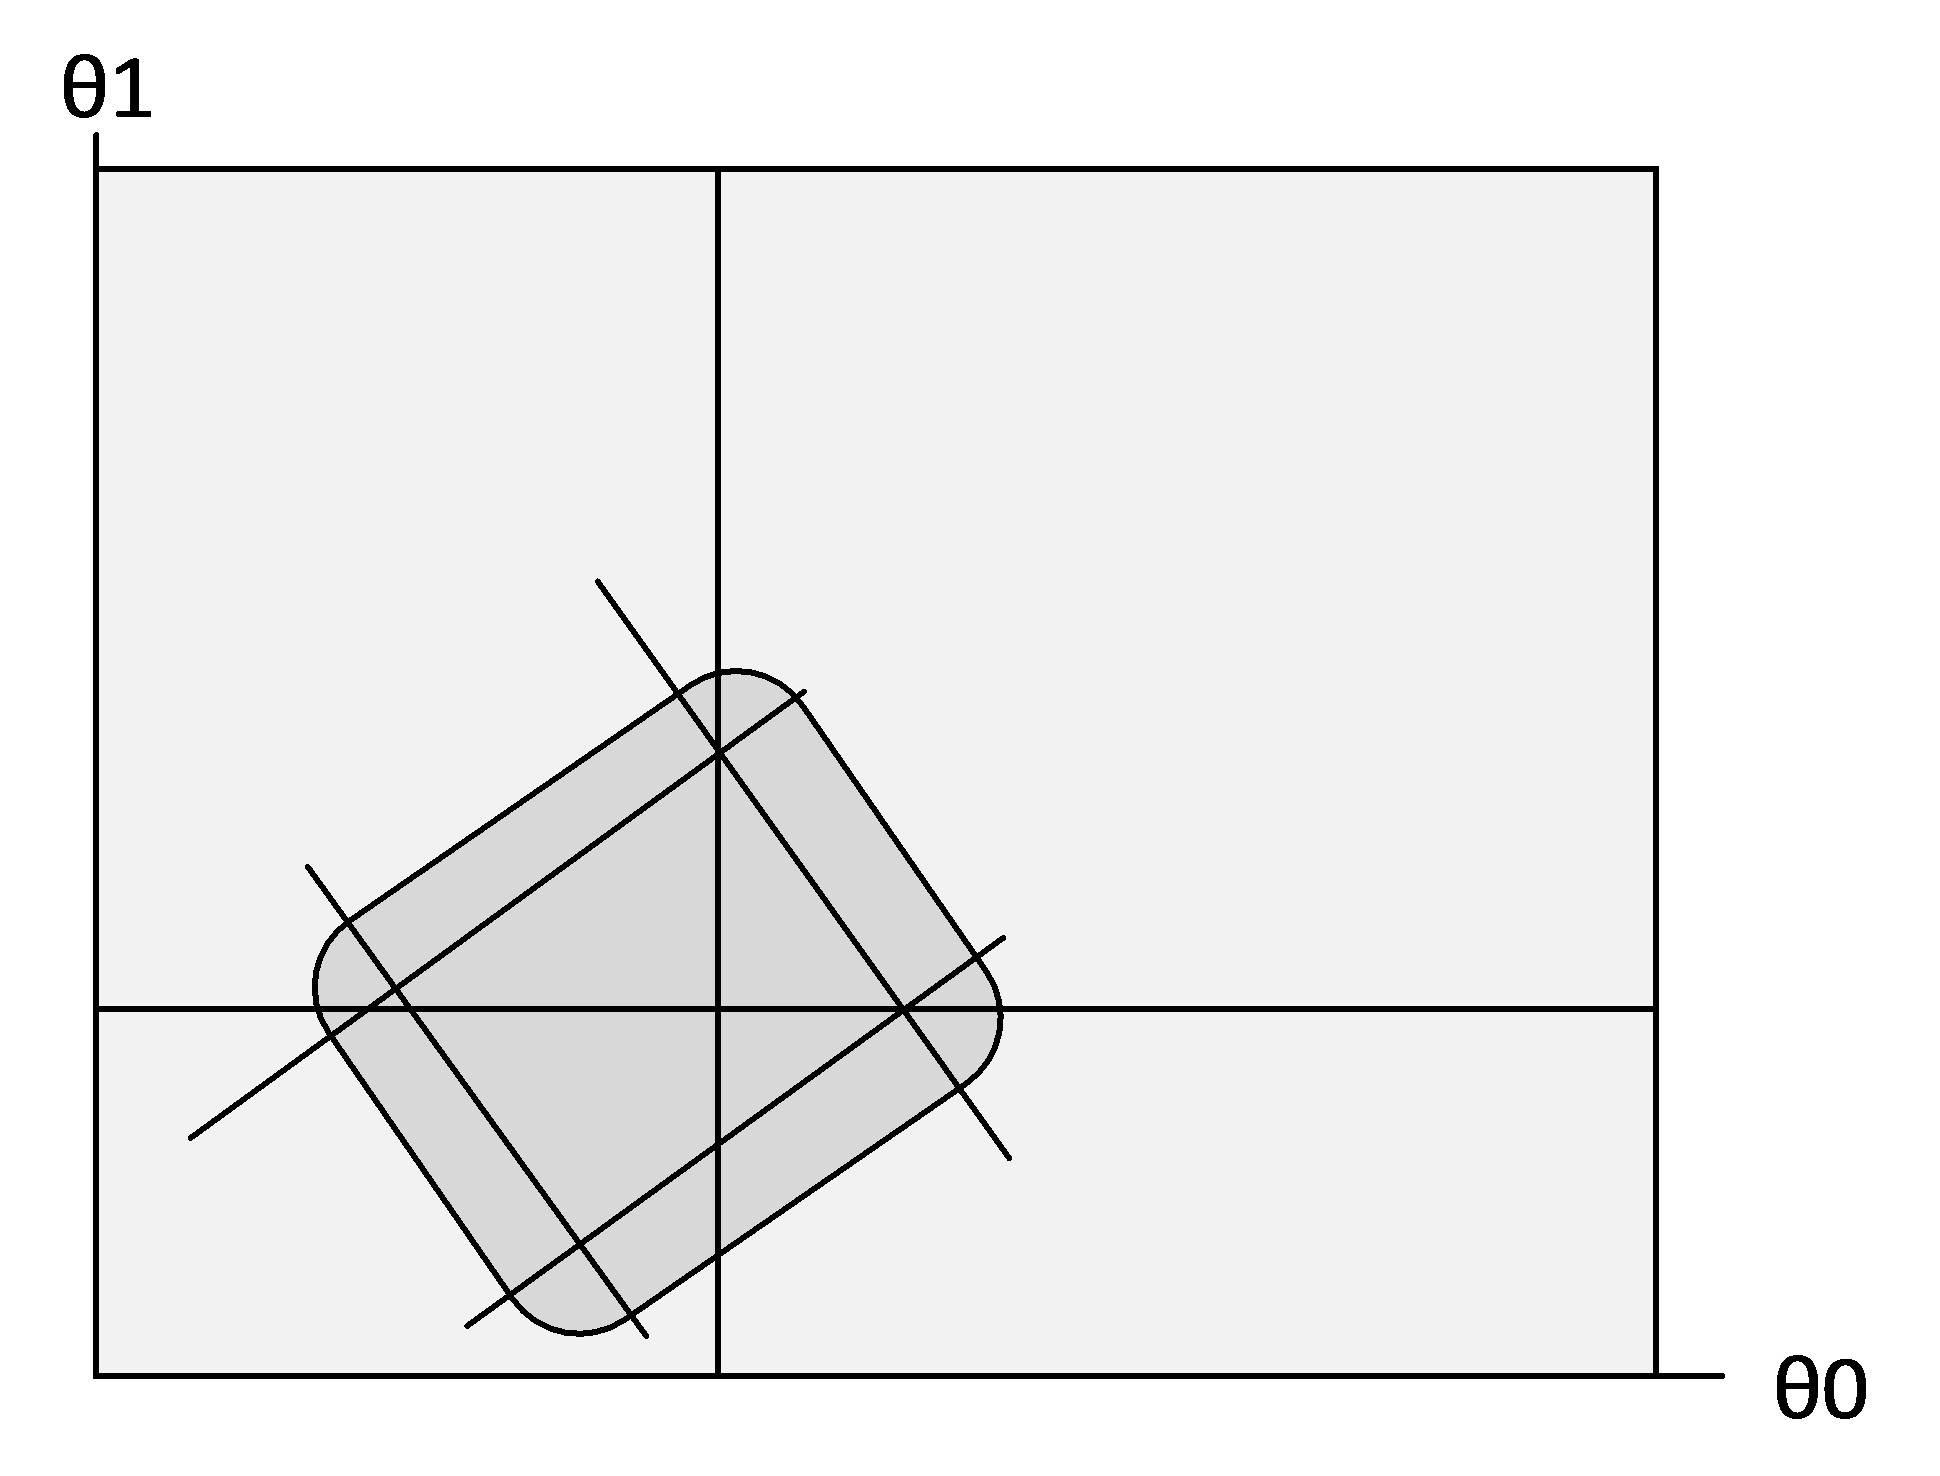
\includegraphics[scale=0.18]{Figure_9.jpg}}
\end{center}
\end{figure}	
\end{frame}
%%%%%%%%%%%%%%%%%%%%%%%%%
\begin{frame}
\frametitle{Inference for the Identified Set}

\begin{itemize}
	\item This procedure is based on Chernozhukov, Hong and Tamer (Econometrica, 2007).
	\item Steps of the procedure:
	\begin{itemize}
		\item (1) At $\theta\in\widehat{\Theta}_{I}^{\varepsilon }$, compute R draws $\{q^{r}(\theta); r=1,\dots,R\}$ such that:
		\begin{equation*}
		q_{r}(\theta)=chol(\widehat{\Omega}_{I,S}(\theta))N(0_{S},I_{S}),
		\end{equation*}
		with
		\begin{equation*}
		\widehat{\Omega }_{I,S}(\hat{\theta})=diag(\widehat{\Sigma}_{I,S}(\hat{\theta}))^{-\frac{1}{2}}\widehat{\Sigma}_{I,S}(\hat{\theta})diag(\widehat{\Sigma}_{I,S}(\hat{\theta}))^{-\frac{1}{2}}.
		\end{equation*}
		Note that we are taking draws from the asymptotic distribution of the normalized recentered moments, evaluated at each point $\theta$.
	\end{itemize}
\end{itemize}
\end{frame}
%%%%%%%%%%%%%%%%%%%%%%%%%
\begin{frame}
\frametitle{Inference for the Identified Set}

\begin{itemize}
	\item Steps of the procedure (cont.)
	\begin{itemize}
		\item (2) Compute one of the following T-statistic for each value of $\theta$ and draw $r$:
		\begin{equation*}
		\begin{split}
		T^{N}_{r}(\theta)&=\sum_{s=1}^{S}(\min\{0,q_{r,s}(\theta)\})^{2}\\
		T^{MS}_{r}(\theta)&=\sum_{s=1}^{S}\{(\min\{0,q_{r,s}(\theta)\})^{2}\times SF^{MS}_{I,s}(\theta)\}\\
		T^{SM}_{r}(\theta)&=\sum_{s=1}^{S}\{(\min\{0,q_{r,s}(\theta)\})^{2} + SF^{SM}_{I,s}(\theta)\}
		\end{split}
		\end{equation*}
		\item (3) For each draw $r$, take the maximum across $\theta$:
		\begin{equation*}
		T^{\max}_{r}=\max_{\theta\in\widehat{\Theta}_{n}^{\varepsilon}}T^{k}_{r}(\theta),\quad k=\{N, MS, SM\}.
		\end{equation*}
	\end{itemize}
\end{itemize}
\end{frame}
%%%%%%%%%%%%%%%%%%%%%%%%%
\begin{frame}
\frametitle{Inference for the Identified Set}

\begin{itemize}
	\item Steps of the procedure (cont.)
	\begin{itemize}
		\item (4) Compute the critical value $c_{\alpha}$ as the $1-\alpha$ quantile of the distribution of $\{T^{\max}_{r}; r=1,\dots,R\}$.
		\item (5) Return to the larger grid of theta points, $\widehat{\Theta }_{n}^{Grid}$, and calculate $T^{obs}(\theta)$ at each candidate value $\theta\in\widehat{\Theta}_{n}^{Grid}$:
		\begin{equation*}
		T^{obs}(\theta)=\sum_{s=1}^{S}(\min\{0,\frac{\overline{m}_{I,s}(\theta)}{\hat{\sigma} _{I,s}(\theta)}\})^{2}
		\end{equation*}
		\item (6) Compare $T^{obs}(\theta)$ against $c_{\alpha}$ and accept $\theta$ into the confidence set whenever $T^{obs}(\theta)$ $<$ $c_{\alpha}$.
	\end{itemize}
\end{itemize}
\end{frame}
%%%%%%%%%%%%%%%%%%%%%%%%%
\begin{frame}
\frametitle{Inference for the Identified Set: Example}

\begin{figure}[h!]
\begin{center}
\subfigure{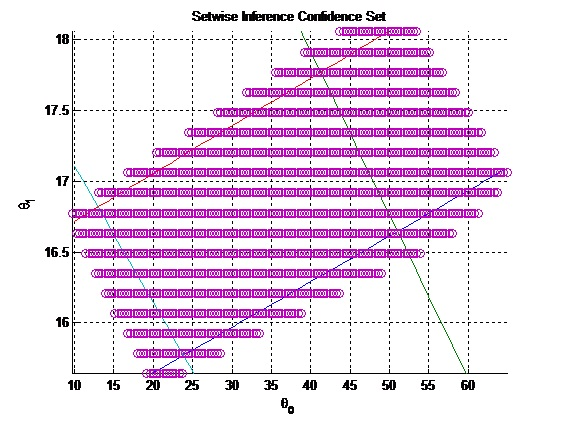
\includegraphics[scale=0.65]{Figure_10.jpg}}
\end{center}
\end{figure}	
\end{frame}
%%%%%%%%%%%%%%%%%%%%%%%%%
\begin{frame}
\frametitle{Inference for the Identified Set: Example}

\begin{figure}[h!]
\begin{center}
\subfigure{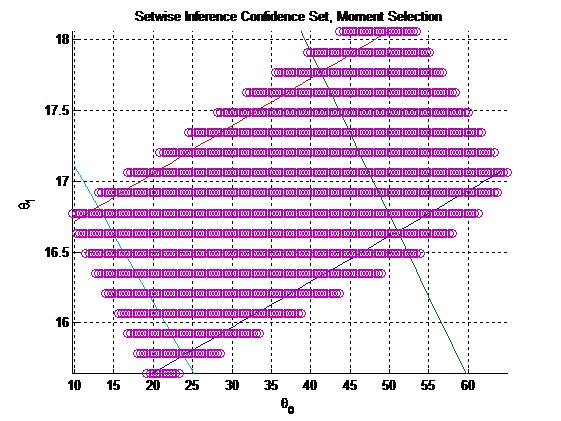
\includegraphics[scale=0.65]{Figure_11.jpg}}
\end{center}
\end{figure}	
\end{frame}
%%%%%%%%%%%%%%%%%%%%%%%%%
\begin{frame}
\frametitle{Inference for the Identified Set: Example}

\begin{figure}[h!]
\begin{center}
\subfigure{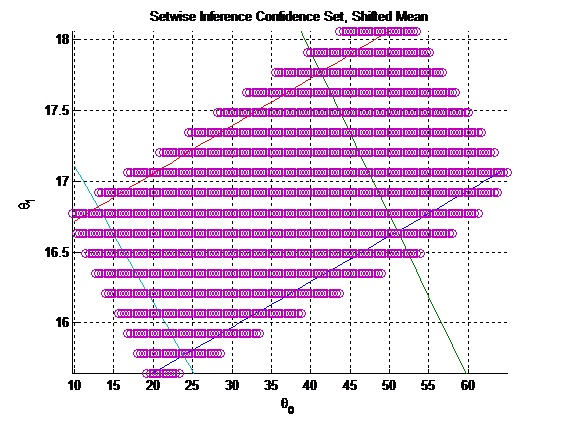
\includegraphics[scale=0.65]{Figure_12.jpg}}
\end{center}
\end{figure}	
\end{frame}
%%%%%%%%%%%%%%%%%%%%%%%%%
\begin{frame}
\frametitle{Inference for the True Parameter}

\begin{itemize}
	\item This procedure is based on Andrews and Soares (Econometrica, 2010).
	\item Steps of the procedure:
	\begin{itemize}
		\item (1) At every $\theta\in\widehat{\Theta}_{n}^{Grid}$, calculate $\{q_{r}(\theta);$ $r=1,\dots,R\}$:
		\begin{equation*}
		q_{r}(\theta)=chol(\widehat{\Omega}_{I,S}(\theta))N(0_{S},I_{S})
		\end{equation*}
		\item (2) For each of these $\theta$ and $r$, calculate: $T_{r}(\theta)$, $T_{r}^{MS}(\theta)$, or $T_{r}^{SM}(\theta)$.
		\item (3) For each $\theta$, calculate the $(1-\alpha)$ quantile. This the critical value, $c(\alpha,\theta)$.
		\item (4) Calculate $T^{obs}(\theta)$ at each candidate value $\theta\in\widehat{\Theta}_{n}^{Grid}$.
		\item (5) Compare $T^{obs}(\theta)$ against $c(\alpha,\theta)$ and accept $\theta$ into the confidence set whenever $T^{obs}(\theta)$ $<$ $c(\alpha,\theta)$.
	\end{itemize}
\end{itemize}
\end{frame}
%%%%%%%%%%%%%%%%%%%%%%%%%
\begin{frame}
\frametitle{Inference for the Identified Set: Example}

\begin{figure}[h!]
\begin{center}
\subfigure{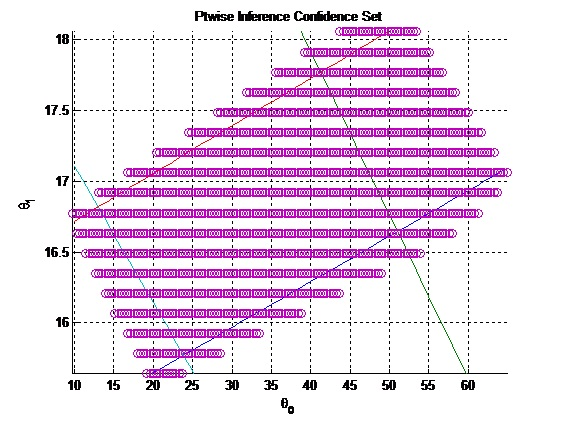
\includegraphics[scale=0.65]{Figure_13.jpg}}
\end{center}
\end{figure}	
\end{frame}
%%%%%%%%%%%%%%%%%%%%%%%%%
\begin{frame}
\frametitle{Inference for the Identified Set: Example}

\begin{figure}[h!]
\begin{center}
\subfigure{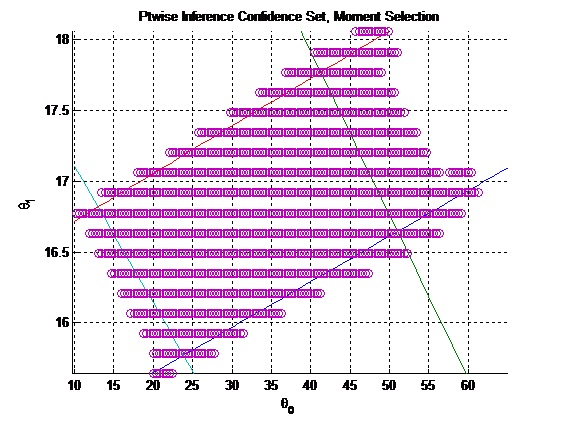
\includegraphics[scale=0.65]{Figure_14.jpg}}
\end{center}
\end{figure}	
\end{frame}
%%%%%%%%%%%%%%%%%%%%%%%%%
\begin{frame}
\frametitle{Inference for the Identified Set: Example}

\begin{figure}[h!]
\begin{center}
\subfigure{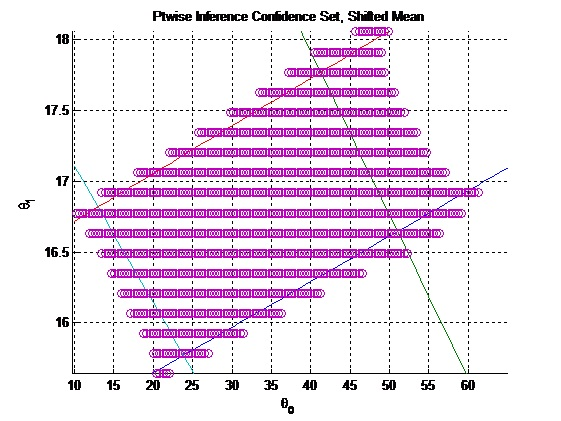
\includegraphics[scale=0.6]{Figure_15.jpg}}
\end{center}
\end{figure}	
\end{frame}
%%%%%%%%%%%%%%%%%%%%%%%%%
\begin{frame}
\frametitle{Comparison of Inference Procedures}

\begin{figure}[h!]
\begin{center}
\subfigure{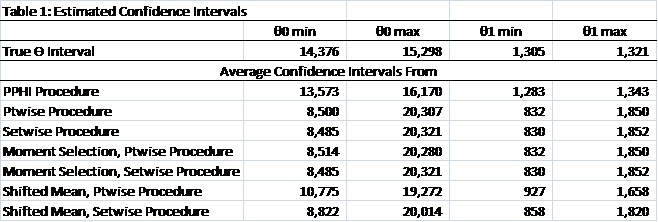
\includegraphics[scale=0.65]{Figure_16.jpg}}
\end{center}
\end{figure}	
\end{frame}

\end{document}